\documentclass{beamer}
\usetheme{Boadilla}
% \renewcommand{\baselinestretch}{1.5}

\usepackage{unicode-math}
\usepackage{physics} % better derivative writings
\usepackage{ulem}
\usepackage{xcolor}
\usepackage{amsmath}

\NewDocumentCommand{\e}{}{\symrm{e}}
\DeclareMathOperator\cis{cis}

\title{Taylor \sout{Swift} Series (Maclaurin Series)}
\author{Kutay}
\institute{Made with LaTeX}
\date{\today}

% \parskip=10pt

% \setkomafont{disposition}{\normalfont\bfseries}

\begin{document}

\begin{frame}
  \titlepage
\end{frame}

\begin{frame}
  \frametitle{Outline}
  \tableofcontents
\end{frame}

\section{What is it?}

\begin{frame}
  \frametitle{What is it?}
  \begin{itemize}
    \item Approximation of a function with an infinite series
    \item Approximates near \( x = 0 \)
  \end{itemize}
\end{frame}

\section{Why?}

\begin{frame}
  \frametitle{Why?}
  \begin{itemize}
    \item To compute \( \sin x \), \( \cos x \), and \( \e^x \) \textit{fast}
    \item Calculators (your TI) use this technique
    \item To simplify equations/functions
    \item In simple pendulum, we \textit{approximated} \( \sin x \) with \( x \)
  \end{itemize}
\end{frame}

\section{Derivation}

\begin{frame}
  \frametitle{Derivation}
  \begin{itemize}
    \item Calculators can multiply, add, subtract, divide, and take powers of whole numbers \textit{quickly}
    \item Using \textit{polynomials} will be efficient
    \item Since polynomials are just multiplications, additions, and exponentiations of numbers
  \end{itemize}
\end{frame}

\begin{frame}
  \frametitle{Derivation}
  \begin{figure}[ht]
    \centering
    \caption{The Function \( \cos x \)}
    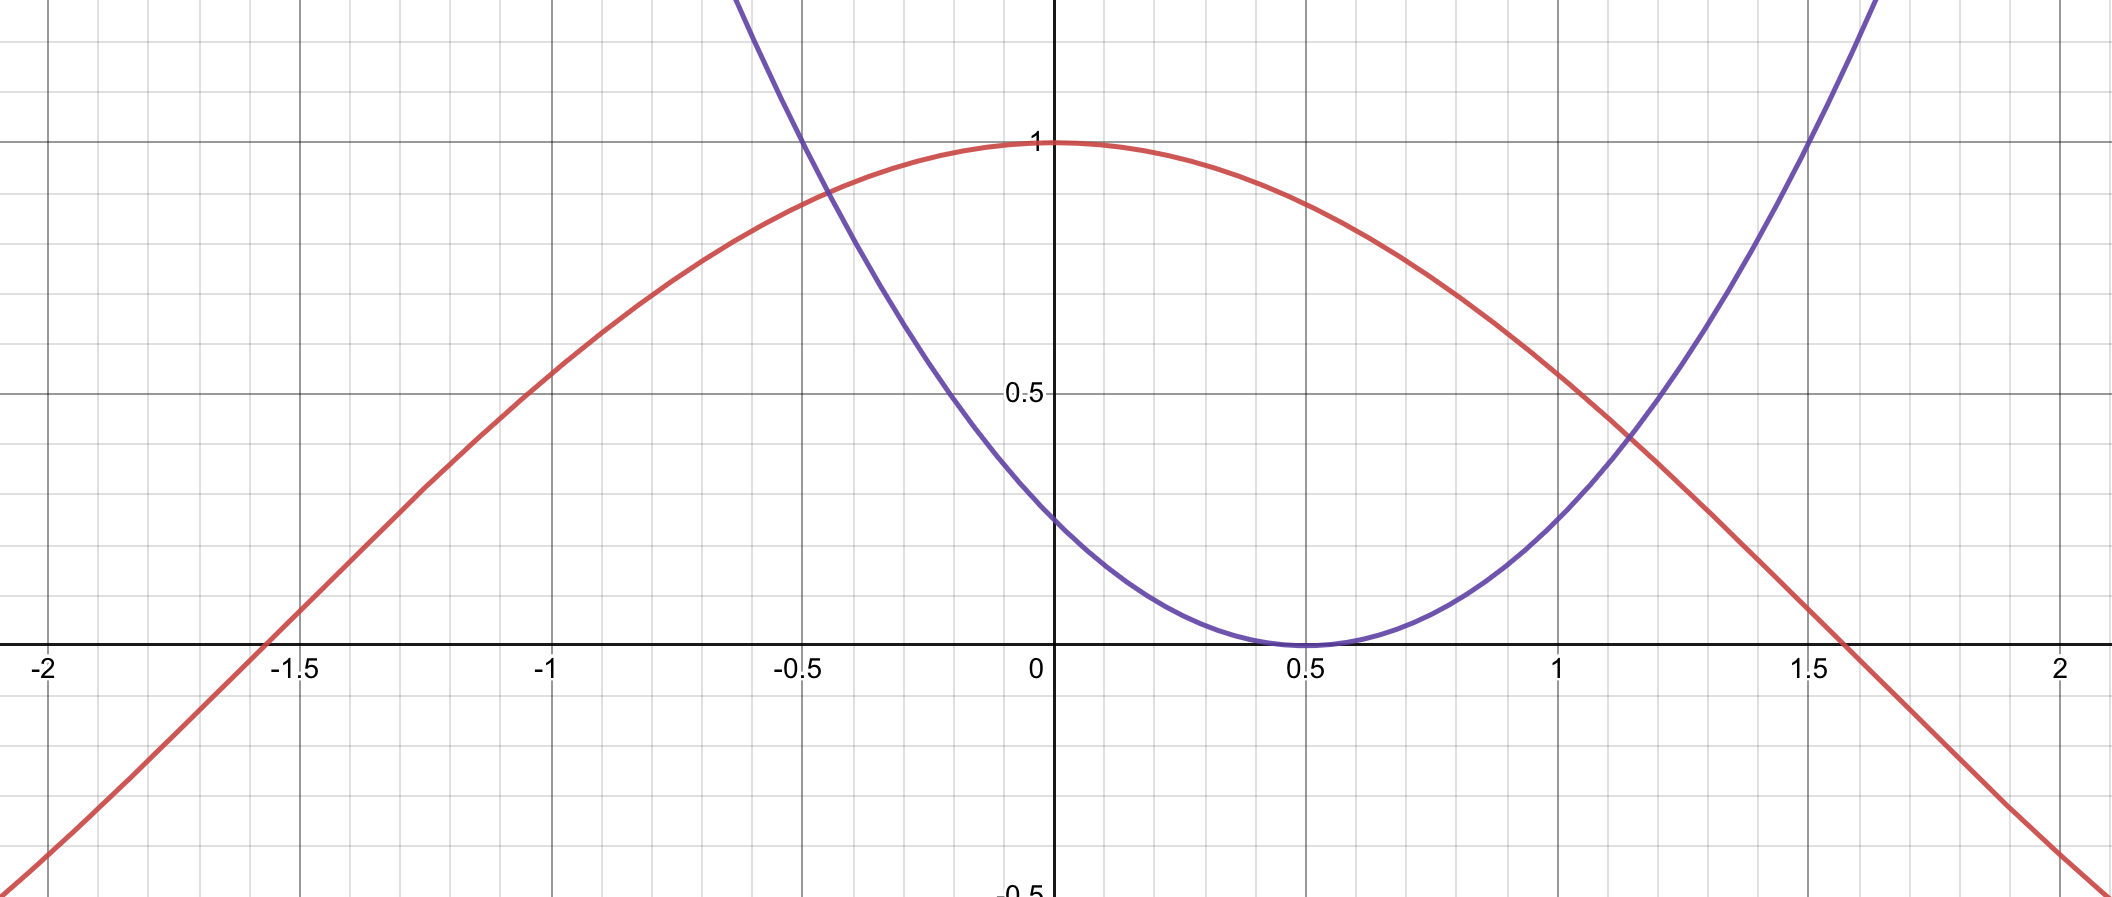
\includegraphics[
      scale=0.13
    ]{images/cosx.png}
  \end{figure}
  \begin{itemize}
    \item Approximate to two degrees
    \item Find real numbers for \( c_0, c_1, \) and \( c_2 \) that approximate \( \cos x \) the \textit{best}
  \end{itemize}
  \begin{equation*}
    \cos x \approx c_0 + c_1x + c_2x^2
  \end{equation*}
\end{frame}

\begin{frame}
  \frametitle{Derivation}
  \begin{itemize}
    \item Approximation \textit{near} \( x = 0 \)
  \end{itemize}
  \begin{align*}
    \cos 0 &= c_0 + c_1 \cdot 0 + c_2 \cdot 0^2 \\
    c_0 & = 1
  \end{align*}
  \begin{figure}[ht]
    \centering
    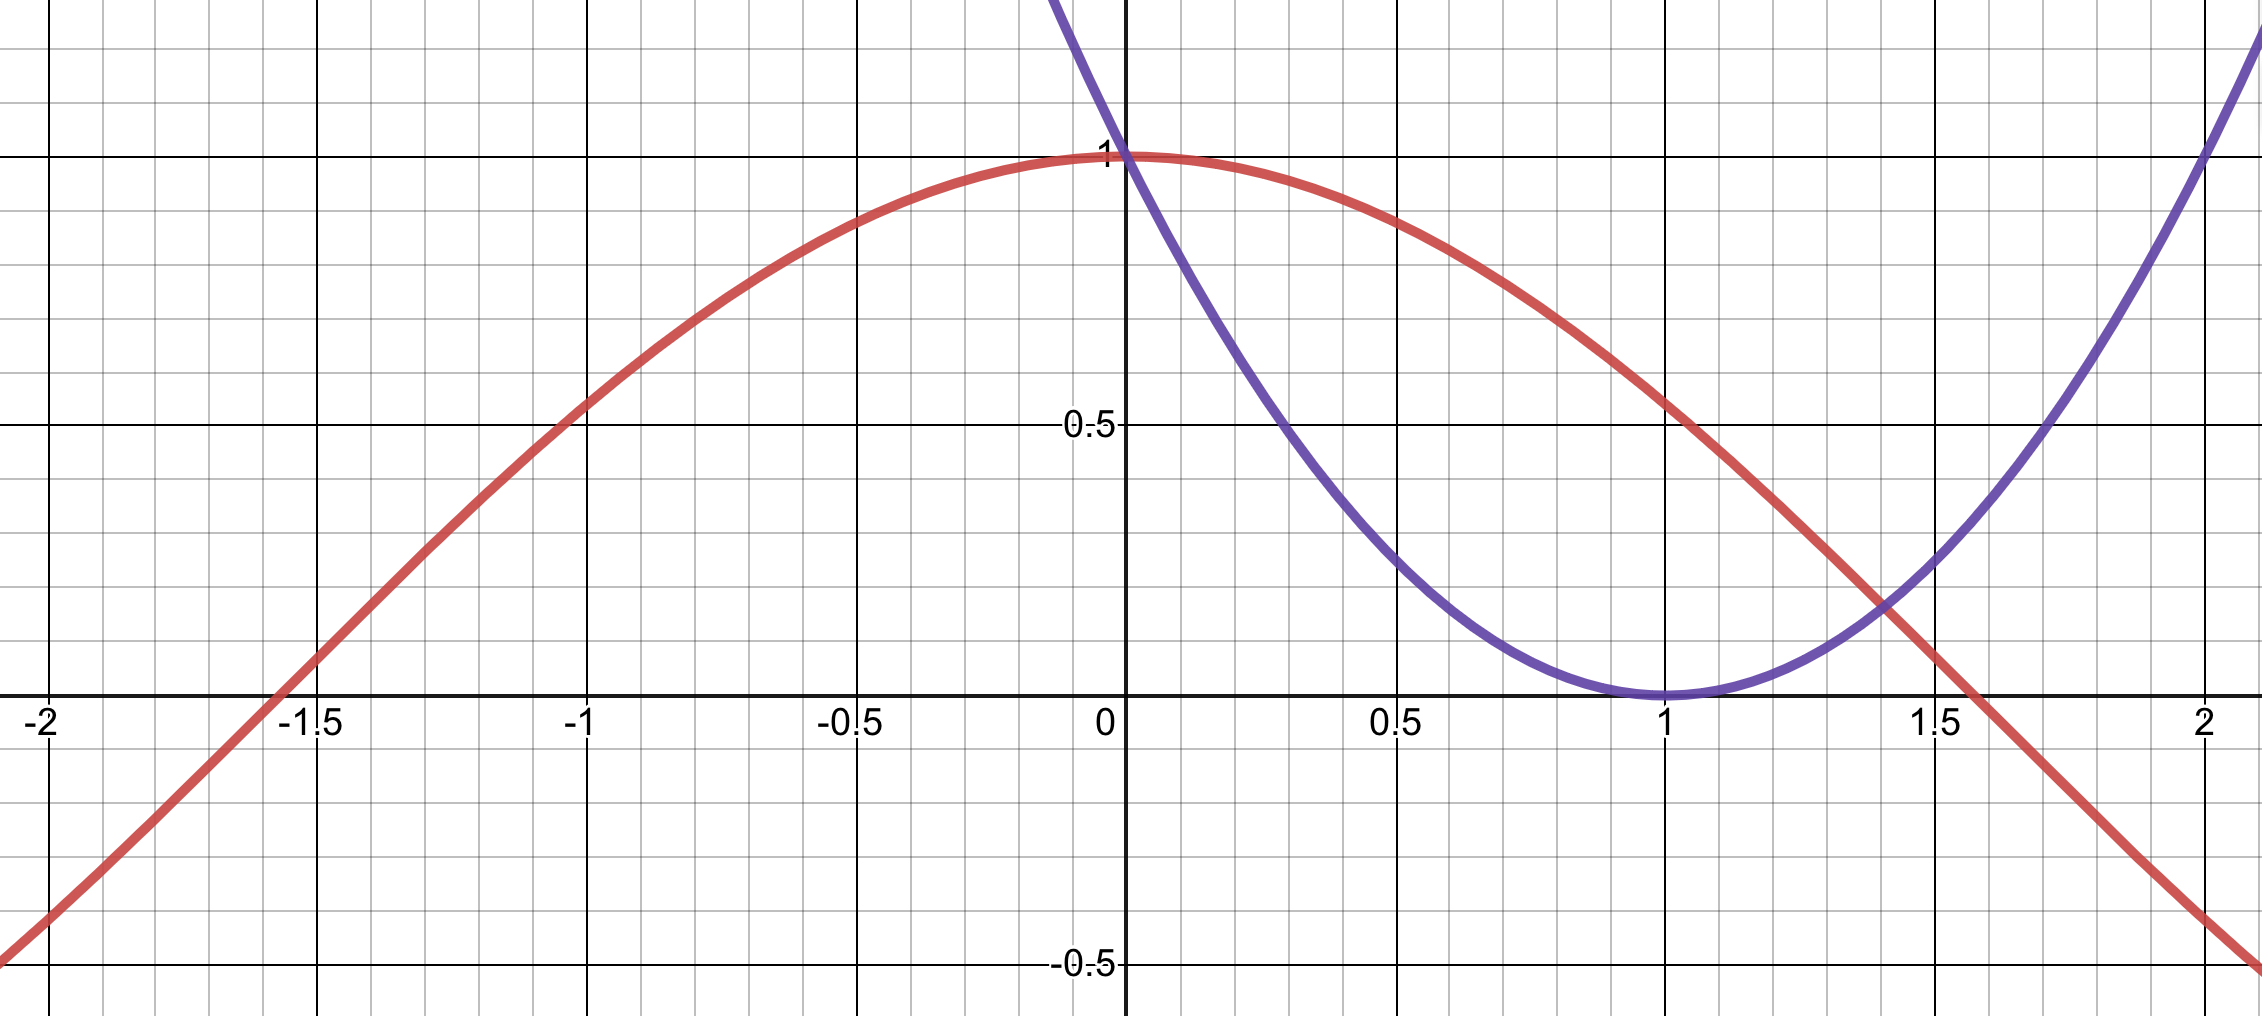
\includegraphics[
      scale=0.15
    ]{images/first.png}
  \end{figure}
\end{frame}

\begin{frame}
  \frametitle{Derivation}
  \begin{figure}[ht]
    \centering
    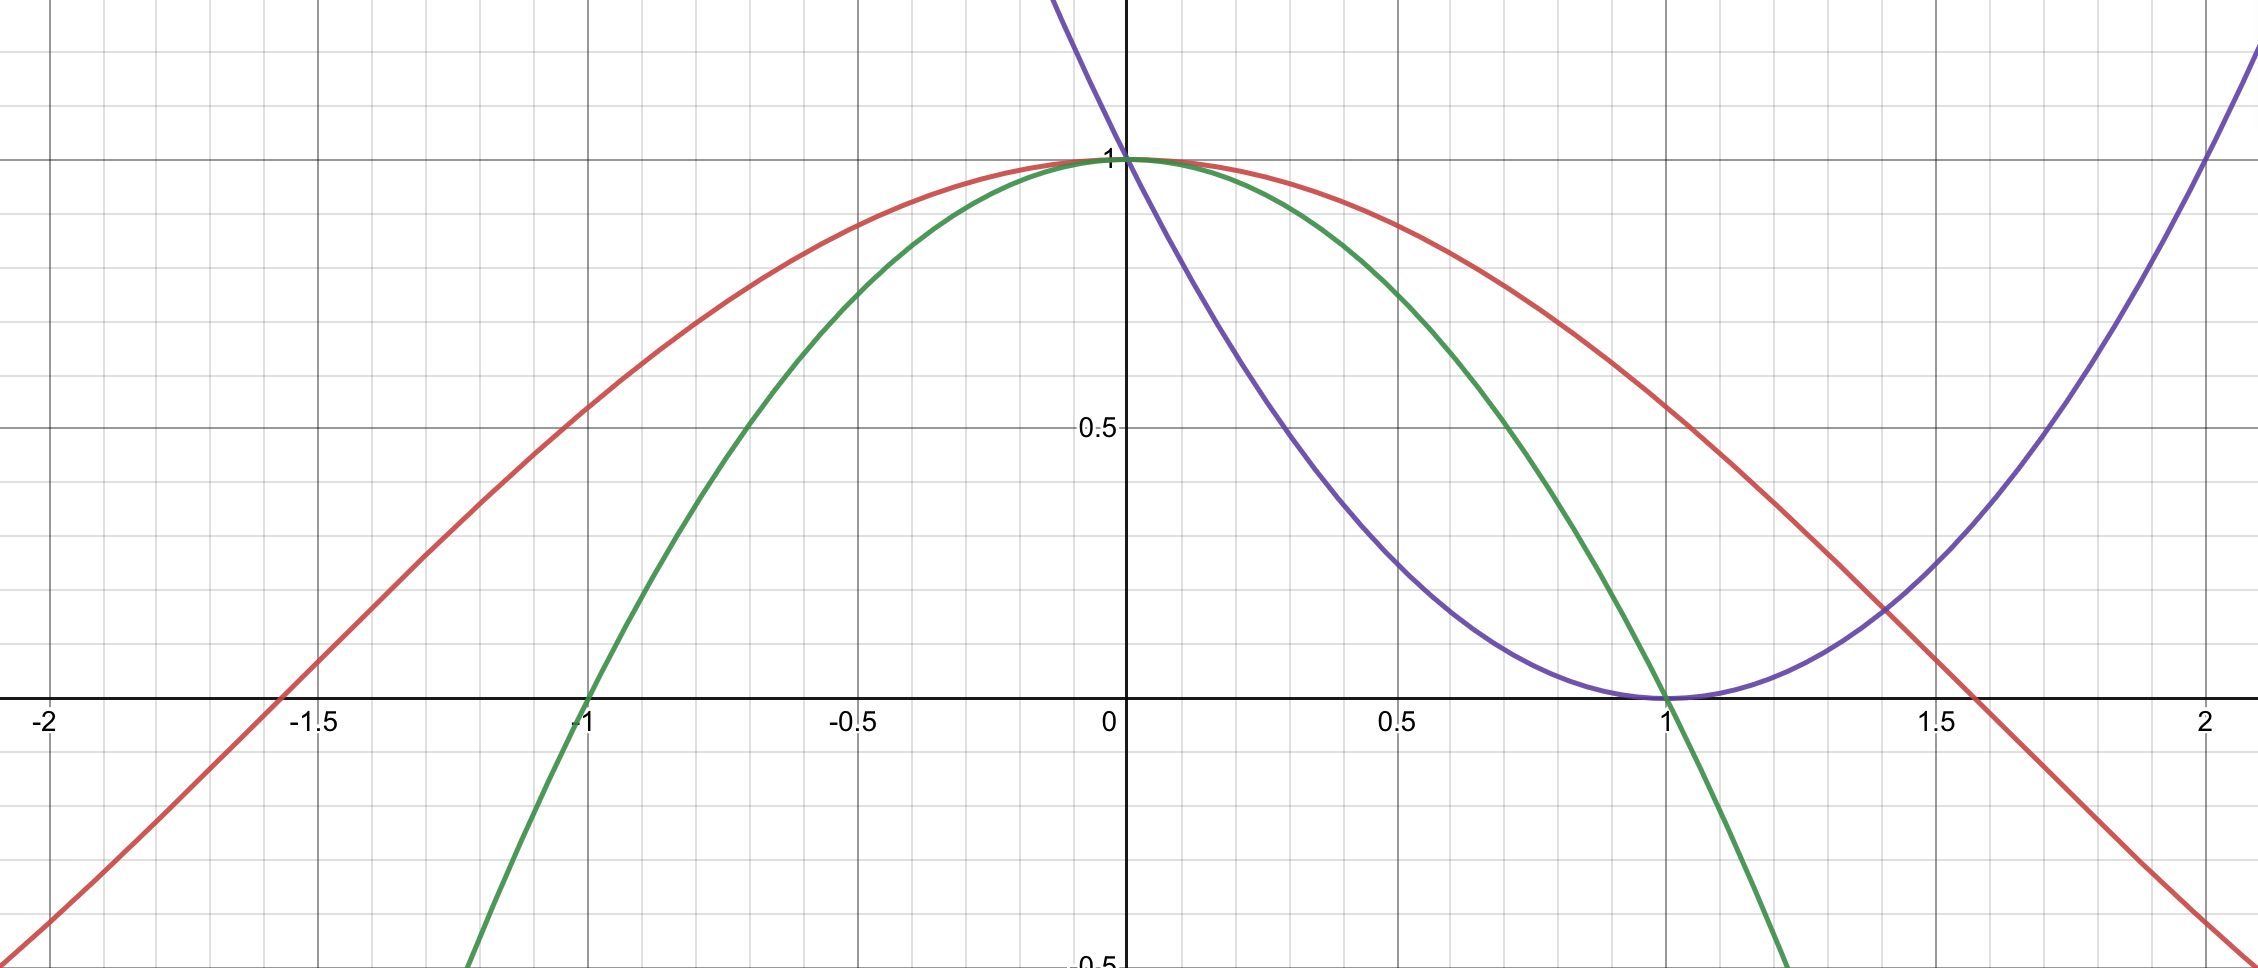
\includegraphics[
      scale=0.12
    ]{images/second.png}
  \end{figure}
  \begin{itemize}
    \item The green function is better, but why?
    \item The rate of change is the same as \( \cos x \) at \( x = 0 \)
    \item Approximation must have the same rate of change at \( x = 0 \)
    \item \( \cos'(x) = -\sin x \), and \( (c_0 + c_1x + c_2x^2)' = c_1 + 2c_2x \)
  \end{itemize}
  \begin{align*}
    -\sin 0 = 0 &= c_1 + 2c_2 \cdot 0 \\
    c_1 &= 0
  \end{align*}
\end{frame}

\begin{frame}
  \frametitle{Derivation}
  \begin{figure}[ht]
    \centering
    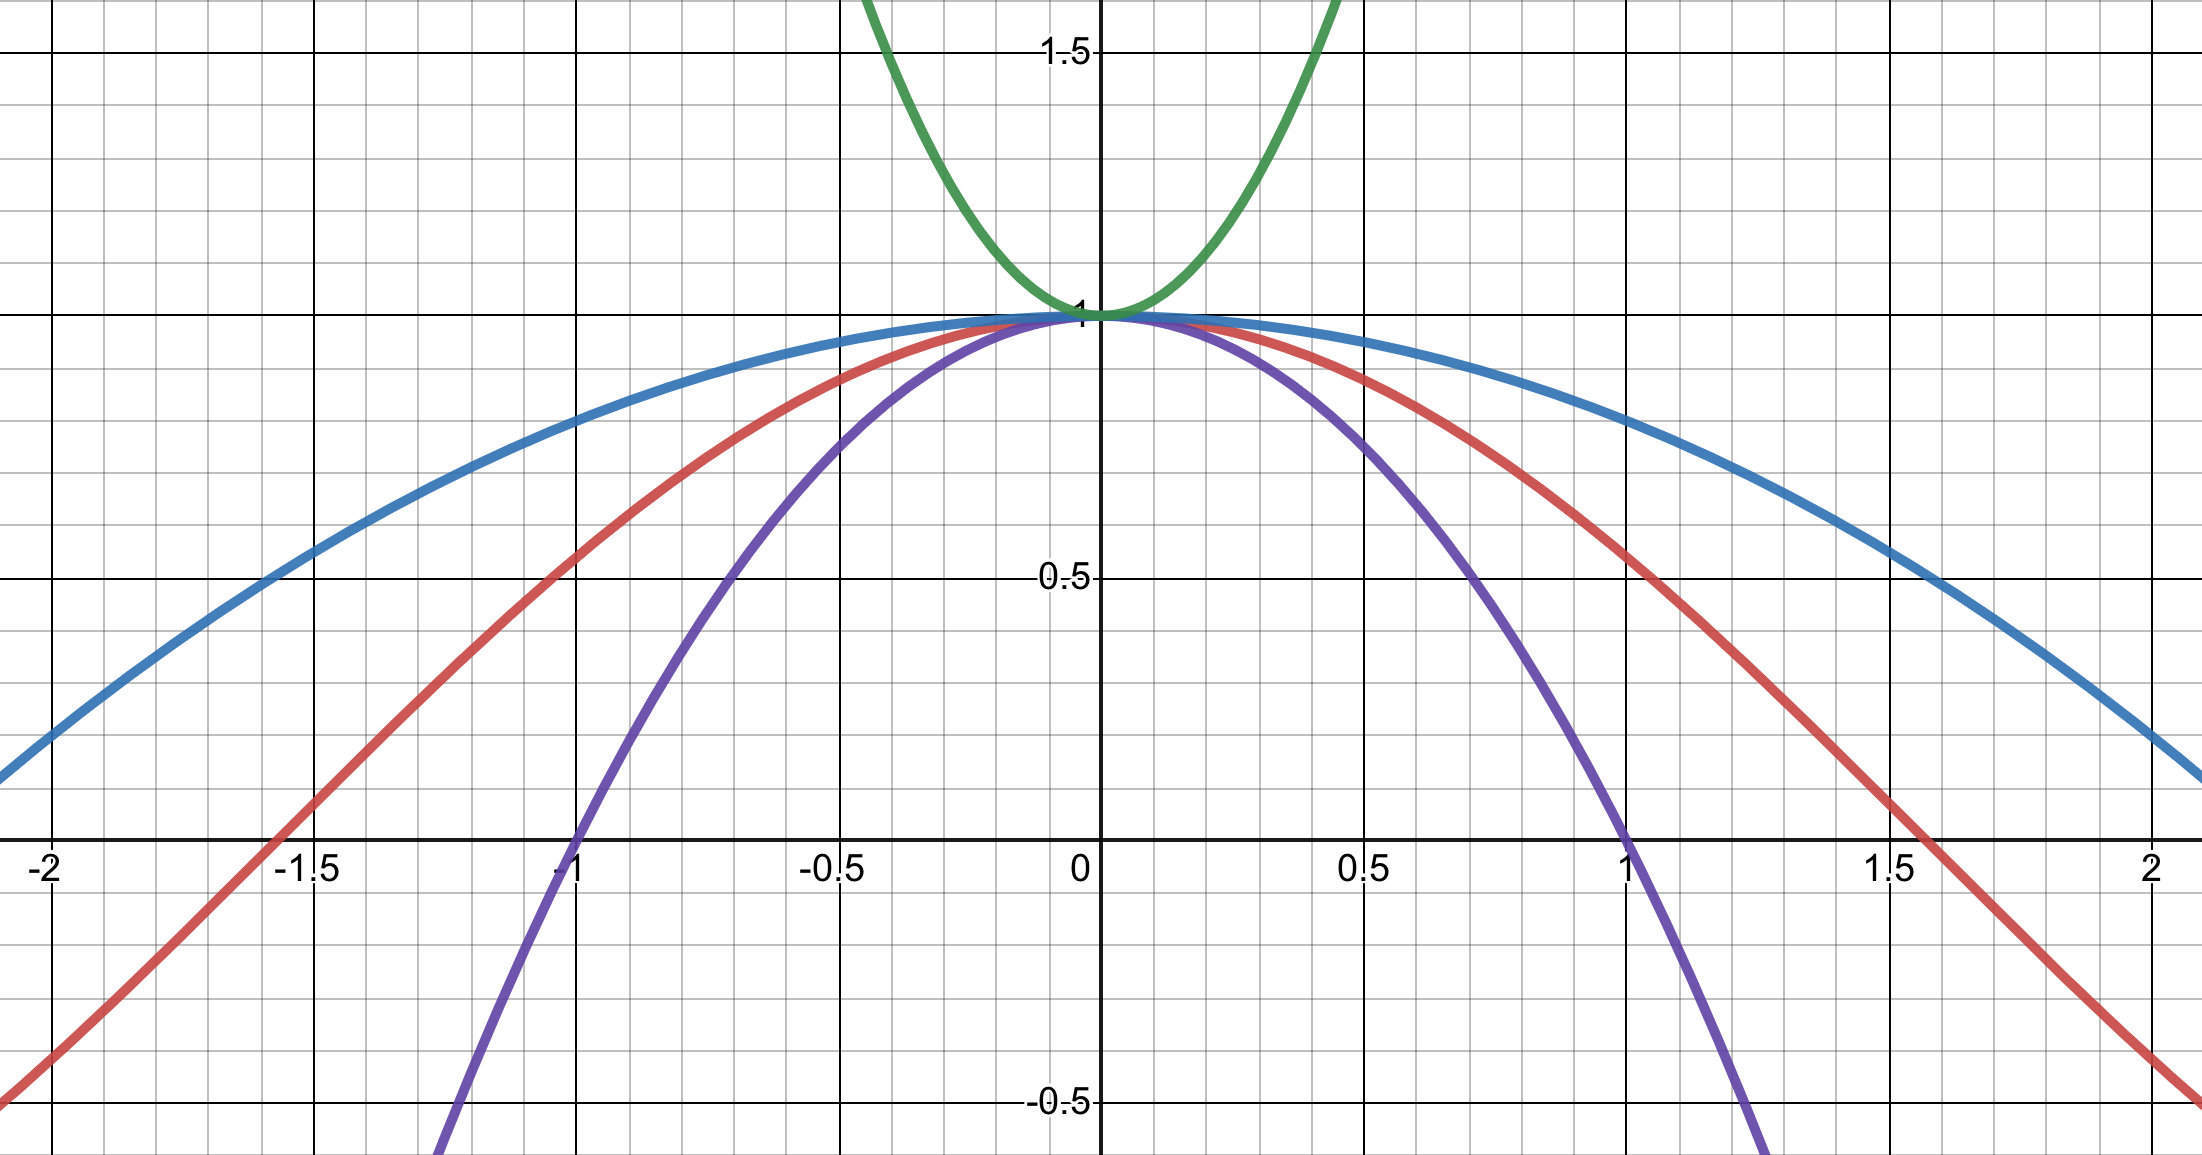
\includegraphics[
      scale=0.1
    ]{images/examples.png}
  \end{figure}
  \begin{itemize}
    \item \( \cos x \) \textit{curves} downwards at \( x = 0 \)
    \item So, the second derivative is negative
    \item So, the rate of change is decreasing
    \item Same second derivative will ensure that they curve at the same rate
  \end{itemize}
  \begin{align*}
    \cos''(x) &= -\cos x \\
    \left(c_0 + c_1x + c_2x^2\right)'' &= 2c_2
  \end{align*}
\end{frame}

\begin{frame}
  \frametitle{Derivation}
  \begin{itemize}
    \item \( \cos''(x) = -\cos x \), and \( \left(c_0 + c_1x + c_2x^2\right)'' = 2c_2 \)
  \end{itemize}
  \begin{align*}
    -\cos 0 &= 2c_2 \\
    -1 &= 2c_2 \\
    c_2 &= -\frac{1}{2} \\
    \cos x &\approx 1 - \frac{1}{2}x^2
  \end{align*}
  \begin{figure}[ht]
    \centering
    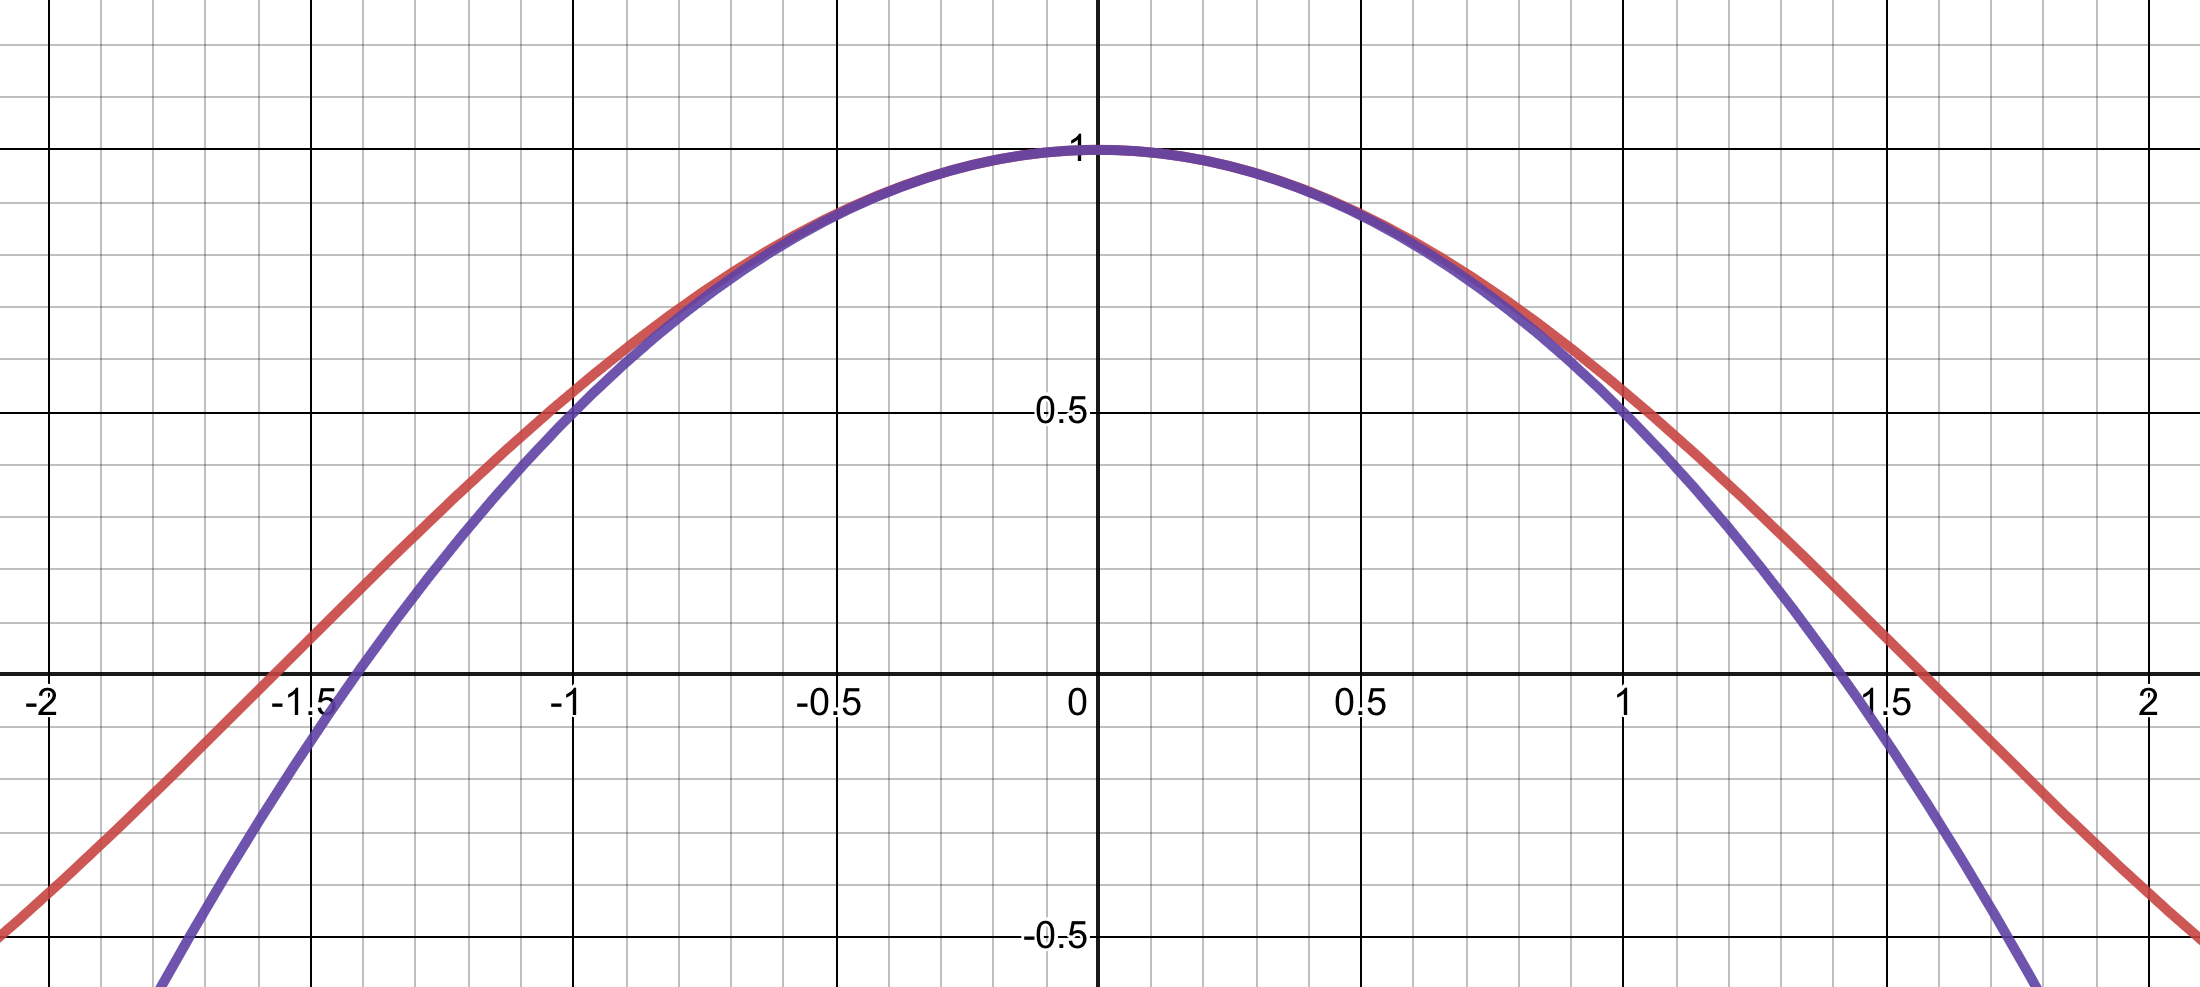
\includegraphics[
      scale=0.115
    ]{images/approx.png}
  \end{figure}
\end{frame}

\begin{frame}
  \frametitle{Derivation}
  \begin{itemize}
    \item Okay, but how \textit{good} is the approximation?
    \item For \( x = 0.1 \), \( \cos x = 0.99500417 \), and the approximation, \( 1 - \frac{1}{2}x^2 = 0.995 \)
    \item For \( x = 0.25 \), \( \cos x = 0.9689124 \), and the approximation, \( 1 - \frac{1}{2}x^2 = 0.96875 \)
  \end{itemize}
  \begin{figure}[ht]
    \centering
    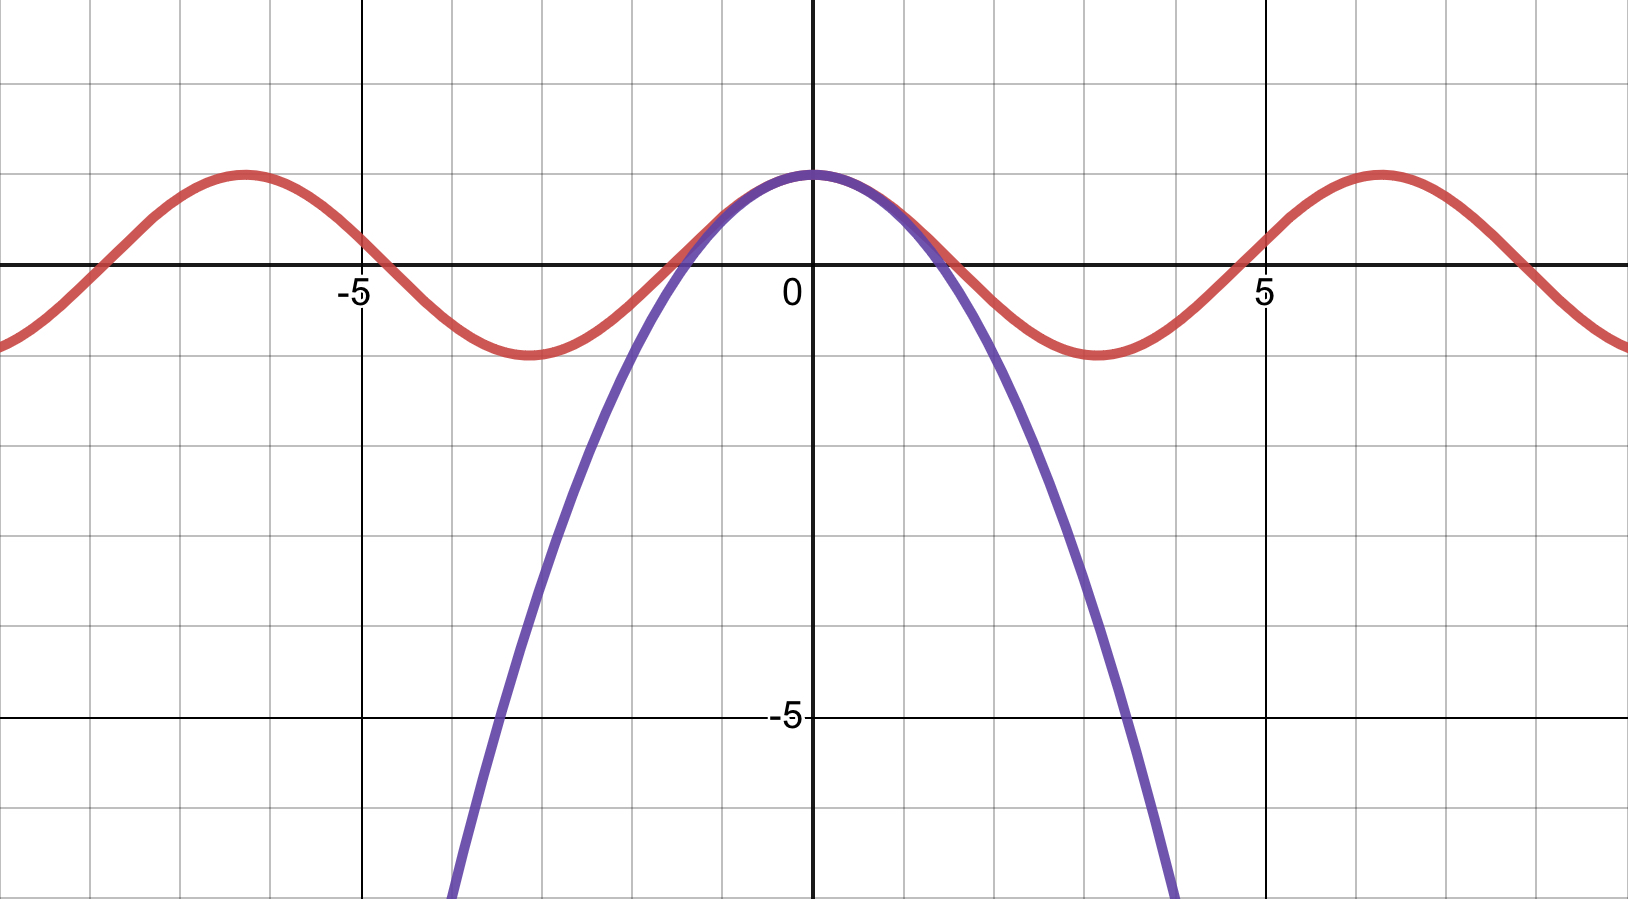
\includegraphics[
      scale=0.16
    ]{images/big.png}
  \end{figure}
\end{frame}

\section{The More the Merrier}

\begin{frame}
  \frametitle{The More the Merrier}
  \begin{itemize}
    \item But why stop at \( x^2 \)? Why not go further?
    \item More terms will give more \textit{control} over the approximation
    \item Add another term \( c_3x^3 \) to the approximation
  \end{itemize}
  \begin{equation*}
    \cos x \approx 1 - \frac{1}{2}x^2 + c_3x^3
  \end{equation*}
  \begin{itemize}
    \item Taking the third derivative of a polynomial, all the terms that have a power less than 3 will vanish
    \item And, \( \cos'''(x) = \sin x \)
    \item Taking the derivative,
  \end{itemize}
  \begin{gather*}
    \cos'''(x) = \sin x = \left(-x + 3c_3x^2\right)'' = \left(-1 + 2 \cdot 3c_3x\right)' = 1 \cdot 2 \cdot 3 \cdot c_3 \\
    \sin 0 = 1 \cdot 2 \cdot 3 \cdot c_3 \\
    c_3 = 0
  \end{gather*}
\end{frame}

\begin{frame}
  \frametitle{The More the Merrier}
  \begin{equation*}
    \cos x \approx 1 - \frac{1}{2}x^2
  \end{equation*}
  \begin{itemize}
    \item This approximation is the best for all cubic polynomials, as well as all the quadratic polynomials
    \item But, we can do better if we extend to another term
  \end{itemize}
  \begin{equation*}
    \cos x \approx 1 - \frac{1}{2}x^2 + c_4x^4
  \end{equation*}
  \begin{align*}
    \cos^{(4)}(x) &= \cos x \\
    \left(1 - \frac{1}{2}x^2 + c_4x^4\right)^{(4)} &= 1 \cdot 2 \cdot 3 \cdot 4 \cdot c_4 \\
    \cos 0 & = 1 \cdot 2 \cdot 3 \cdot 4 \cdot c_4 \\
    c_4 & = \frac{1}{24}
  \end{align*}
\end{frame}

\begin{frame}
  \frametitle{The More the Merrier}
  \begin{equation*}
    \cos x \approx 1 - \frac{1}{2}x^2 + \frac{1}{24}x^4
  \end{equation*}
  \begin{figure}[ht]
    \centering
    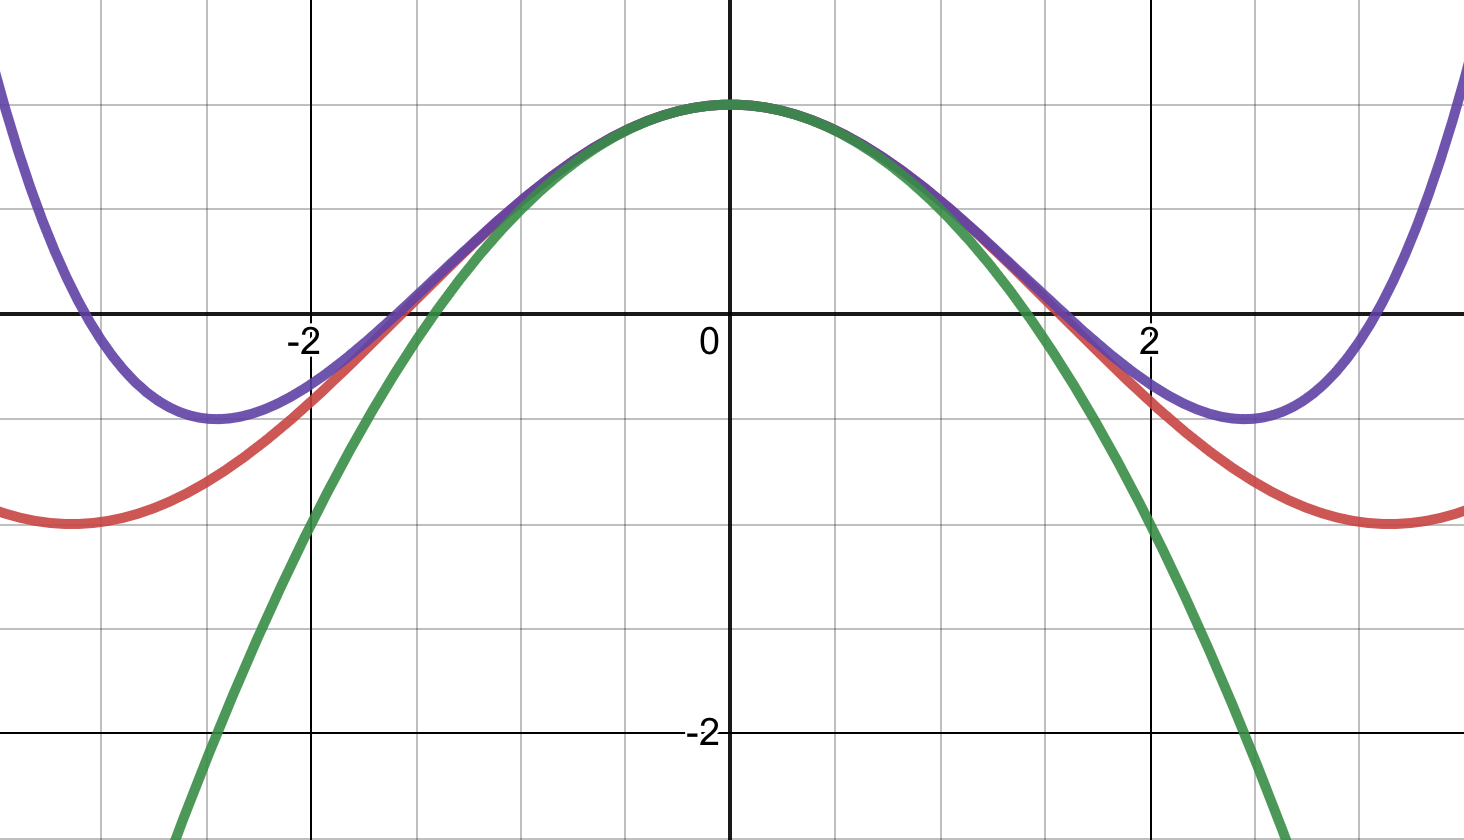
\includegraphics[
      scale=0.17
    ]{images/better.png}
  \end{figure}
  \begin{itemize}
    \item This is a really good approximation of \( \cos x \)
    \item For most physics problems, this would be fine
    \item But, we are dealing with maths
  \end{itemize}
\end{frame}

\section{Notice a Few Things}

\begin{frame}
  \frametitle{Notice a Few Things}
  \begin{itemize}
    \item Firstly, factorials come up quite naturally from taking \( n \) successive derivatives of \( c_nx^n \)
  \end{itemize}
  \begin{align*}
    \dv{\left(c_nx^n\right)}{x} &= n \cdot c_n \cdot x^{n - 1} \\
    \dv[2]{\left(c_nx^n\right)}{x} &= n \cdot (n - 1) \cdot c_n \cdot x^{n - 2} \\
    \dv[3]{\left(c_nx^n\right)}{x} &= n \cdot (n - 1) \cdot (n - 2) \cdot c_n \cdot x^{n - 3} \\
    & \vdots \\
    \dv[n]{\left(c_nx^n\right)}{x} &= n! \cdot c_n
  \end{align*}
  \begin{itemize}
    \item So, we have to divide by the appropriate factorial to cancel out this effect
  \end{itemize}
  \begin{equation*}
    c_n = \frac{\text{desired derivative value}}{n!}
  \end{equation*}
\end{frame}

\begin{frame}
  \frametitle{Notice a Few Things}
  \begin{itemize}
    \item Secondly, adding new terms does \textit{not} mess up older terms
    \item Other higher-order terms that have \( x \) will not affect the lower order terms
  \end{itemize}
  \begin{align*}
    P(x) & = 1 - \frac{1}{2}x^2 + c_4 x^4 \\
    P''(0) & = 2\left(-\frac{1}{2}\right) + 3 \cdot 4 (0)^2
  \end{align*}
  \begin{itemize}
    \item Each derivative of a polynomial at \( x = 0 \) is controlled by one and only one of the coefficients
  \end{itemize}
  \begin{equation*}
    P(x) = c_0 + c_1x + c_2x^2 + c_3x^3 + c_4x^4
  \end{equation*} % controls f(0), f'(0), f''(0), f'''(0), f(n)(0), etc.
\end{frame}

\begin{frame}
  \frametitle{Notice a Few Things}
  \begin{itemize} % What we are doing here is taking information about higher-order derivatives of a
    % function at a single point, and translating that into information about the value of the
    % function near that point
    \item Derivative information at \( x = 0 \) \( \longrightarrow \) output information near \( x = 0 \)
  \end{itemize}
  \begin{figure}[ht]
    \centering
    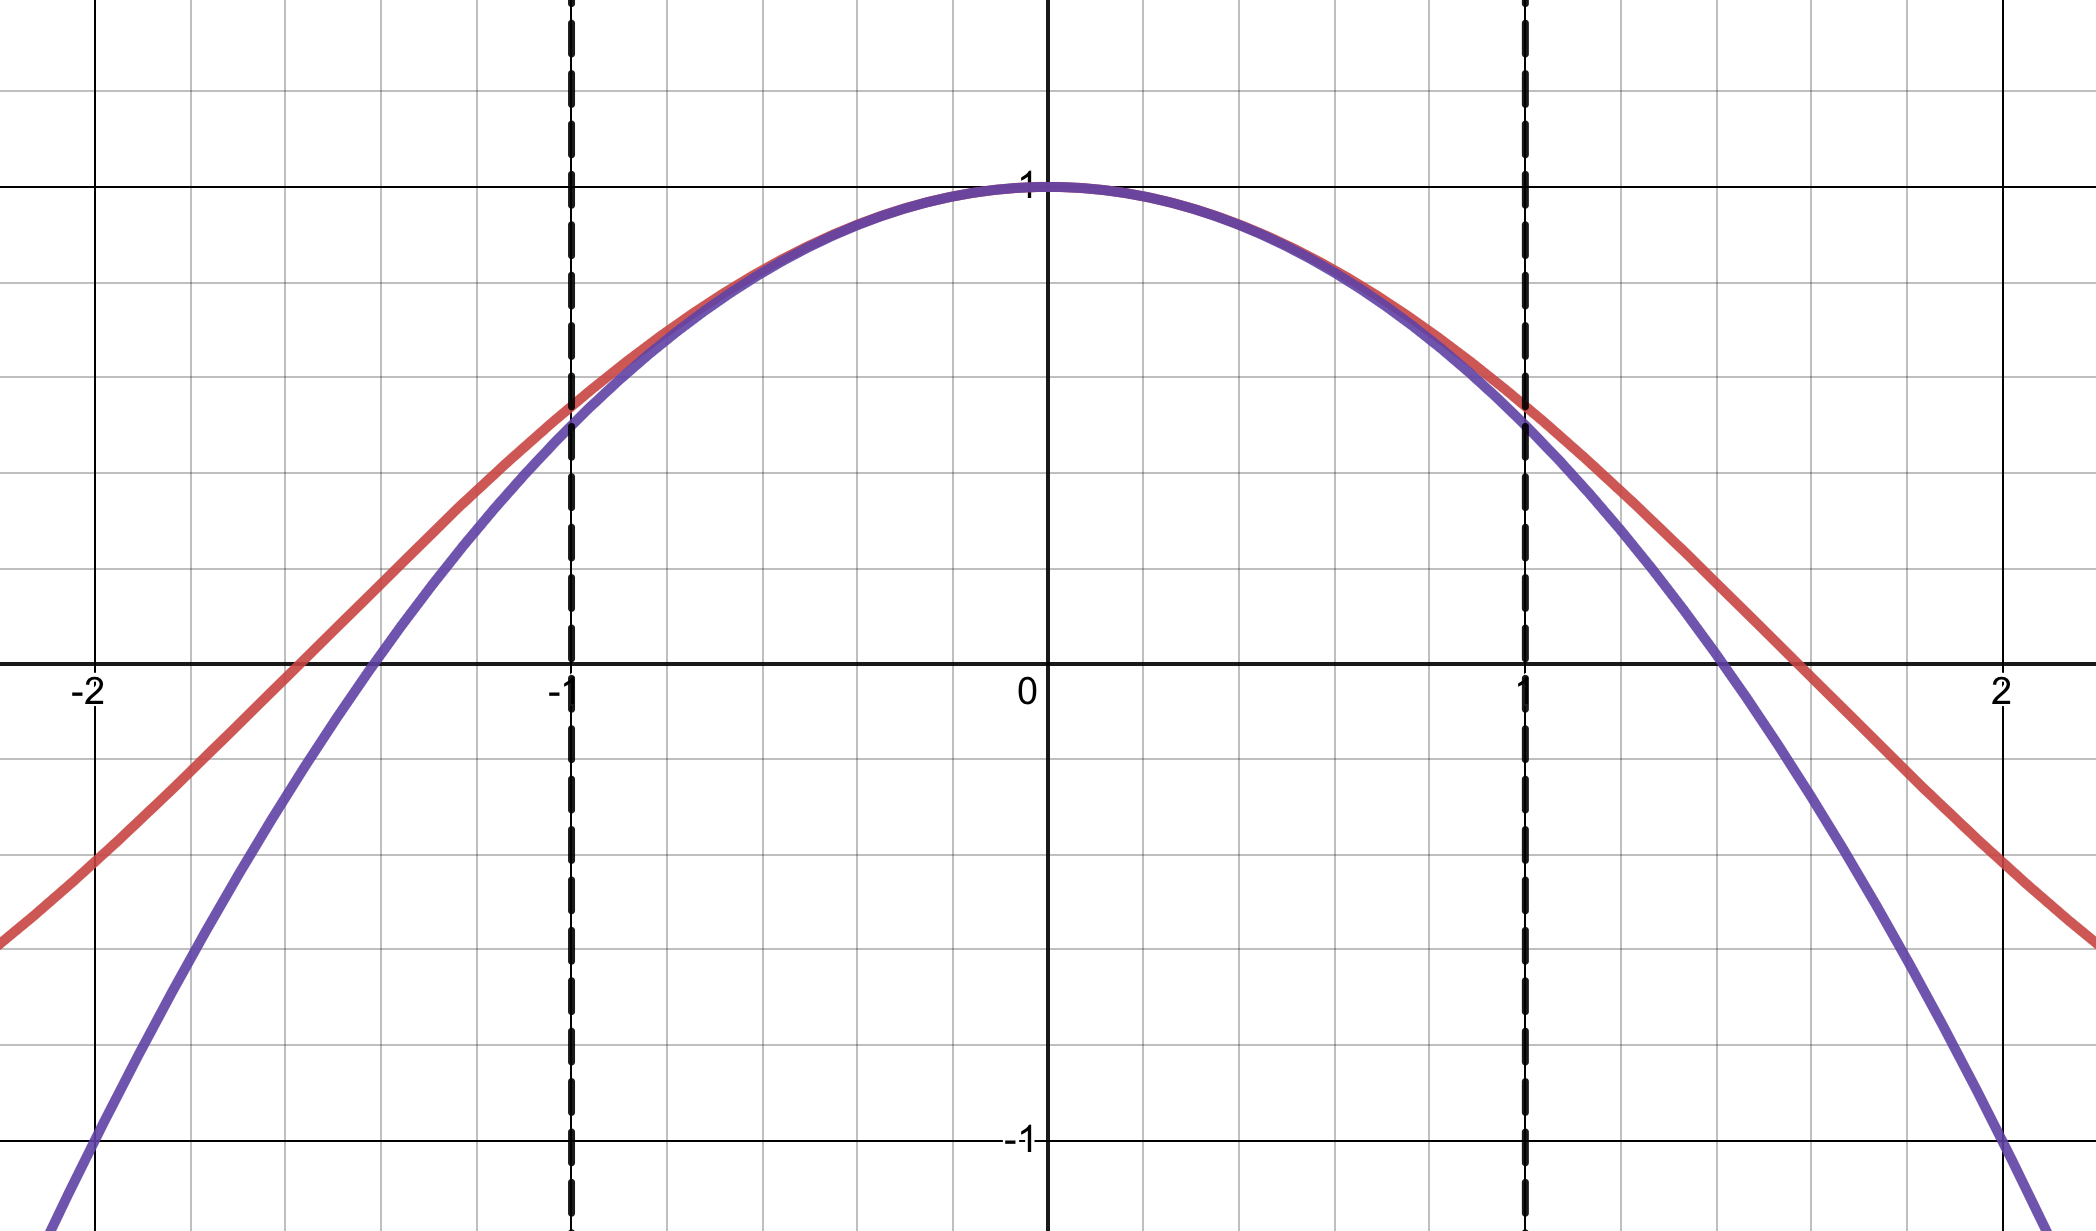
\includegraphics[
      scale=0.13
    ]{images/leverage.png}
  \end{figure}  
\end{frame}

\definecolor{r}{RGB}{210, 15, 57}
\definecolor{b}{RGB}{30, 102, 245}
\definecolor{g}{RGB}{64, 160, 43}
\definecolor{p}{RGB}{136, 57, 239}
\definecolor{o}{RGB}{254, 100, 11}

\begin{frame}
  \frametitle{Notice a Few Things}
  \begin{align*}
    \cos 0 & = \textcolor{r}{1} \\
    \cos' 0 & = \textcolor{b}{0} \\
    \cos'' 0 & = \textcolor{g}{-1} \\
    \cos''' 0 & = \textcolor{p}{0} \\
    \cos^{(4)} 0 & = \textcolor{r}{1} \\
    & \vdots
  \end{align*}
  \begin{equation*}
    P(x) = \textcolor{r}{1} + \textcolor{b}{0}\frac{x^1}{1!} + \textcolor{g}{-1}\frac{x^2}{2!} + \textcolor{p}{0}\frac{x^3}{3!} + \textcolor{r}{1}\frac{x^4}{4!} + \cdots
  \end{equation*}
  \begin{itemize}
    \item Those factorials are there to cancel out the cascading effect of derivatives
  \end{itemize}
\end{frame}

\section{Maclaurin Series}

\begin{frame}
  \frametitle{Maclaurin Series}
  \begin{itemize}
    \item The same approach can be used for \textit{any} function
    \item We can approximate \( f(x) \) near \( x = 0 \) with any degree of accuracy we want
  \end{itemize}
  \begin{equation*}
    P(x) = f(0) + f'(0)\frac{x}{1} + f''(0)\frac{x^2}{2!} + f'''(0)\frac{x^3}{3!} + \cdots = \sum_{n = 0}^{\infty} \frac{f^{(n)}(0)x^n}{n!}
  \end{equation*}
  \begin{itemize}
    \item This summation at infinity is the \textit{Maclaurin series} of \( f(x) \)
    \item Let us approximate the function \( e^x \) (which is in the \textit{Formula Booklet})
  \end{itemize} % one important thing here is that we say that the polynomial converges to our function
\end{frame}

\begin{frame}
  \frametitle{Maclaurin Series}
  \begin{itemize}
    \item Any derivative of \( e^x \) is \( e^x \), so \( e^0 = 1 \)
  \end{itemize}
  \begin{equation*}
    e^x = 1 + x + \frac{x^2}{2!} + \frac{x^3}{3!} + \frac{x^4}{4!} + \cdots
  \end{equation*}
  \begin{figure}[ht]
    \centering
    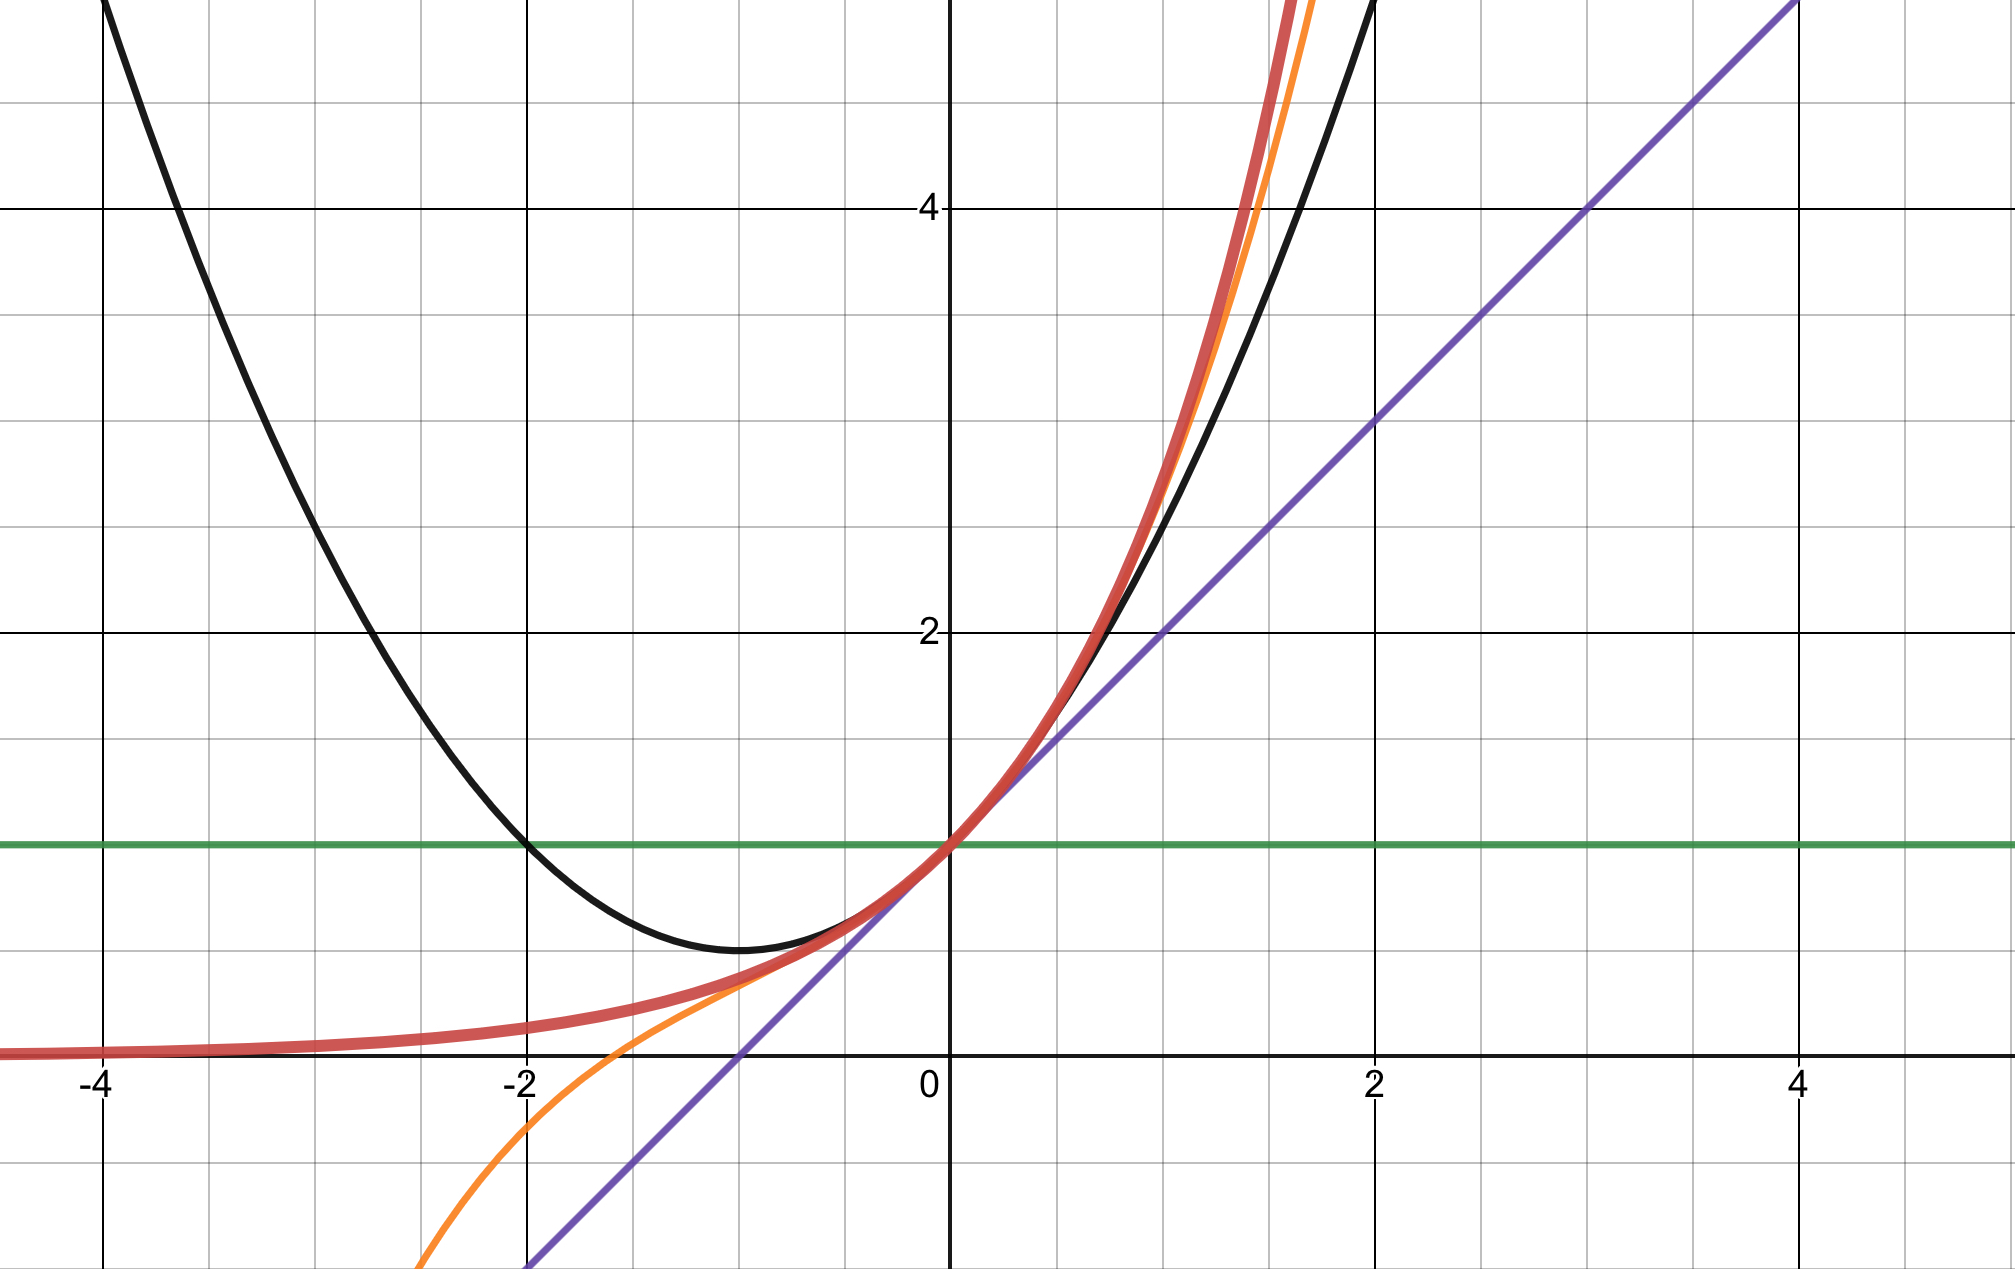
\includegraphics[
      scale=0.14
    ]{images/ex.png}
  \end{figure}
\end{frame} % another thing to notice is that this actually approximates e, plug in x = 1, you would get an approximation of e

\section{Euler's Formula}

\begin{frame}
  \frametitle{Euler's Formula}
  \begin{itemize}
    \item We can, in fact, use this to prove
  \end{itemize}
  \begin{equation*}
    \cos \theta + i\sin \theta = \e^{i\theta}
  \end{equation*}
  \begin{align*}
    \cos \theta & = 1 - \frac{\theta^2}{2!} + \frac{\theta^4}{4!} - \frac{\theta^6}{6!} + \cdots \\
    \sin \theta & = \theta - \frac{\theta^3}{3!} + \frac{\theta^5}{5!} - \frac{\theta^7}{7!} + \cdots \\
    e^{i\theta} & = 1 + (i\theta) + \frac{(i\theta)^2}{2!} + \frac{(i\theta)^3}{3!} + \frac{(i\theta)^4}{4!} + \frac{(i\theta)^5}{5!} + \frac{(i\theta)^6}{6!} + \frac{(i\theta)^7}{7!} + \cdots \\
    & = 1 + i\theta - \frac{\theta^2}{2!} - \frac{i\theta^3}{3!} + \frac{\theta^4}{4!} + \frac{i\theta^5}{5!} - \frac{\theta^6}{6!} - \frac{i\theta^7}{7!} + \cdots \\
    & = \left(1 - \frac{\theta^2}{2!} + \frac{\theta^4}{4!} - \frac{\theta^6}{6!} + \cdots\right) + i\left(\theta - \frac{\theta^3}{3!} + \frac{\theta^5}{5!} - \frac{\theta^7}{7!} + \cdots\right) \\
    & = \cos \theta + i\sin \theta \\
    & = \cis \theta
  \end{align*}
\end{frame}

\section{Example}

\begin{frame}
  \frametitle{Example}
  \begin{itemize}
    \item Find the Maclaurin series of the function \( f(x) = \e^x\sin x \) up to the term \( x^3 \)
    \item Two methods: multiply series expansions of \( \e^x \) and \( \sin x \), or rigor
  \end{itemize}
  \begin{align*}
    f(x) & = \e^x\sin x \\
    f'(x) & = \e^x\sin x + \e^x\cos x \\
    f''(x) & = \e^x\cos x - \e^x\sin x + \e^x\sin x + \e^x\cos x = 2e^x\cos x \\
    f'''(x) & = 2\e^x\cos x - 2\e^x\sin x = 2\e^x(\cos x - \sin x)
  \end{align*}
  \begin{itemize}
    \item \( f(0) = 0 \), \( f'(0) = 1 \), \( f''(0) = 2 \), \( f'''(0) = 2 \)
  \end{itemize}
  \begin{align*}
    f(x) & = 0 + 1x + \frac{2x^2}{2!} + \frac{2x^3}{3!} \\
    & = x + x^2 + \frac{x^3}{3}
  \end{align*}
\end{frame}

\section{Connection to Taylor Series}

\begin{frame}
  \frametitle{Connection to Taylor Series}
  \begin{itemize}
    \item Maclaurin series approximates a function near \( x = 0 \)
    \item Can be approximated near any point \( x = a \) using Taylor series
  \end{itemize}
  \begin{equation*}
    P(x) = f(a) + f'(a)(x - a) + f''(a)\frac{(x - a)^2}{2!} + f'''(a)\frac{(x - a)^3}{3!} + \cdots
  \end{equation*}
  \begin{figure}[ht]
    \centering
    \caption{The Function \( \ln x \) and Approximation}
    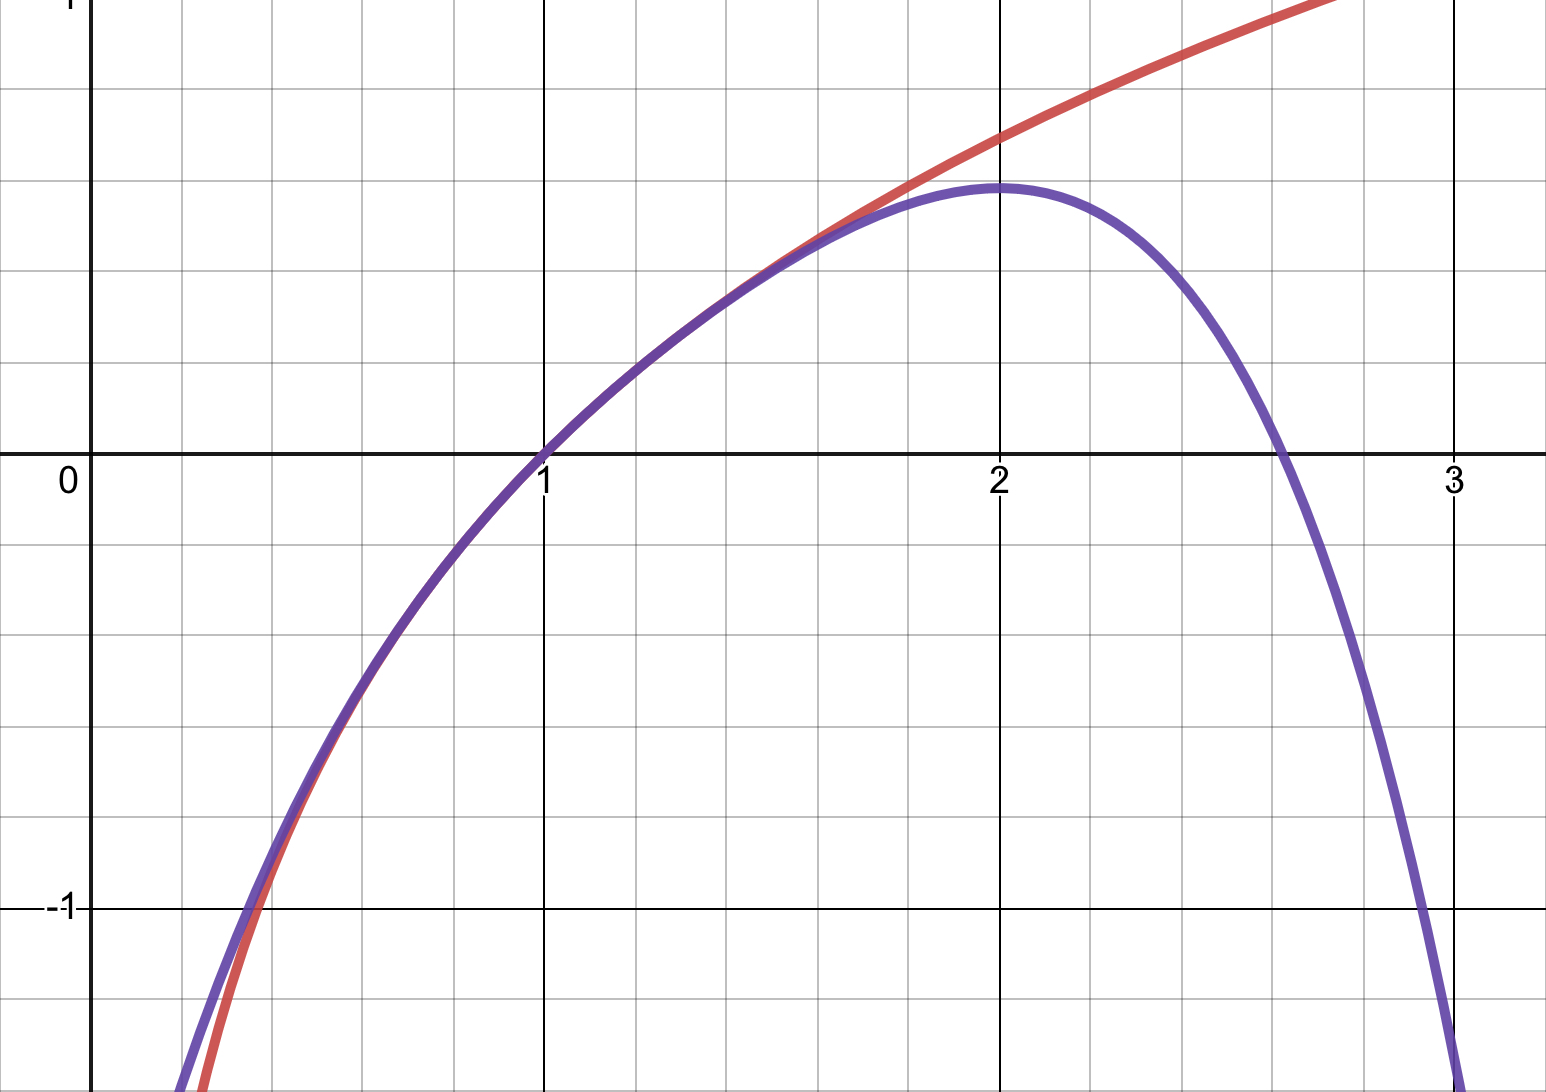
\includegraphics[
      scale=0.13
    ]{images/taylor.png}
  \end{figure}
\end{frame}

\end{document}
